\documentclass[fyp,12pt]{socreport}

% Some generic packets.
\usepackage{color, colortbl}
\usepackage{url}
\usepackage{graphicx}
\usepackage{caption}
\usepackage{subcaption}
\usepackage{pgfplots}
\usepackage{tabularx}
\usepackage{multirow}
\usepackage{listings}
\usepackage{fullpage}
\pgfplotsset{width=10cm,compat=1.9}

% Sets the root path to look for all images.
\graphicspath{{images/}}

% Sets default options for listings.
\renewcommand\lstlistlistingname{List of Listings}
\newcommand*\lstinputpath[1]{\lstset{inputpath=#1}}
\lstinputpath{listings}
\lstset{frame=single, tabsize=2, captionpos=b}
\newcommand{\itab}[1]{\hspace{0em}\rlap{#1}}
\newcommand{\tab}[1]{\hspace{.11\textwidth}\rlap{#1}}

\begin{document}
\pagenumbering{roman}

% Replace as necessary
\title{Development of a Database Link Between Mainframe and PC}
\author{Chua Meng Lee}
\projyear{AY 2016/2017}
\projnumber{H90000}
\advisor{Assoc Prof Jarzabek Stanislaw}
\deliverables{
    \item \itab{Report:} \tab{1 Volume}
    \item \itab{Manual:} \tab{1 Volume}
    \item \itab{Program:} \tab{1 Diskette}
    \item \itab{Database:} \tab{1 Diskette}
}
\maketitle

% Replace as necessary
\begin{abstract}
The use of Wireless Sensor Networks for environmental monitoring has become
increasingly popular over the past decade due to its affordability, ease of deployment
and customisation, as well as its potentiality in the processing of sensed data. One of the
greatest challenges in this field would be in the design and implementation of an
efficient routing protocol which takes into account the various limitations of Wireless
Sensor Networks, such as battery life, limited storage capacities and high probability of
packet losses. Besides this, it is also extremely difficult to evaluate the performance of
such a protocol under crisis scenarios, due to its infrequency and unpredictability. In our
work, we have designed a routing protocol based on optimised Virtual Polar Coordinate
Routing (VPCR) (Newsome and Song, 2003) for use with our three-dimensional
testbed, comprising of 48 MICAz (Crossbow) motes spread across two floors of a
building. We have also developed a Java-based application with features for Event
Emulation and simple nodal analysis to assist us in our experiments. The overall
performance of our protocol will be gauged based on the average Path Stretch Factor
and path length comparisons between optimised and naïve VPCR.

\begin{descriptors}
    \item \itab{C.2.1}	\tab{Network Architecture and Design}
    \item \itab{C.2.2}	\tab{Network Protocols}
    \item \itab{C.2.4}	\tab{Distributed Systems}
    \item \itab{C.4} 	\tab{Performance of Systems}
    \item \itab{I.2.9}	\tab{Robotics}
\end{descriptors}
\begin{keywords}
    Wireless communication, routing protocols, distributed applications, fault tolerance, sensors
\end{keywords}

% Replace/Delete as necessary
\begin{implement}
    Ubuntu Linux 7.04 Feisty Fawn, TinyOS 2.x, NesC 1.2.8a, Java 1.6 SE, Xbow
Motes, Tembusu cluster
\end{implement}

\end{abstract}

% Replace as necessary
\begin{acknowledgement}
See \texttt{README.md} of this repository.
\end{acknowledgement}

\listoffigures % Remove if no figures
\listoftables % Remove if no tables
\lstlistoflistings % Remove if no listings
\tableofcontents

% Actual contents in the contents folder.
% Include additional tex files here.
\chapter{Introduction}
This is the introduction of the example report using LaTex\cite{lamport1986document}. Also an example citation.

\section{Goals}
This is some \textbf{BOLD} text.

This is some \textit{italicised} text.

This is some \texttt{monospaced} text.

This is some math: $a^2 + b^2 = c^2$.

\subsection{Contributions}
This is an example of an enumeration.

\begin{enumerate}
    \item Point one.
    \item Point two.
    \item Point three.
\end{enumerate}

\begin{lstlisting}[
    language=TeX,
    caption={Example Listing.}
]
\title{An Example HYP Final Report}
\author{Harold Finch}
\projyear{2015}
\projnumber{123-45-6789}
\advisor{Dr. Samaritan}
\deliverables{
    \item Report: 1 Volume
}
\maketitle
\end{lstlisting}
\chapter{Results}
REPLACE WITH ACTUAL CONTENTS.

\section{Section 1}

\begin{table}[h]
\centering
\begin{tabular}{|l|l|l|l|}
\hline
         & Scissors & Paper & Stone \\ \hline
Scissors & Draw     & Win   & Lose  \\ \hline
Paper    & Lose     & Draw  & Win   \\ \hline
Stone    & Win      & Lose  & Draw  \\ \hline
\end{tabular}
\caption{Rules for Scissors-Paper-Stone.}
\label{table:example}
\end{table}

Table~\ref{table:example} shows an example table.

\section{Section 2}

\begin{figure}[h]
\centering
\begin{subfigure}[b]{.5\textwidth}
  \centering
  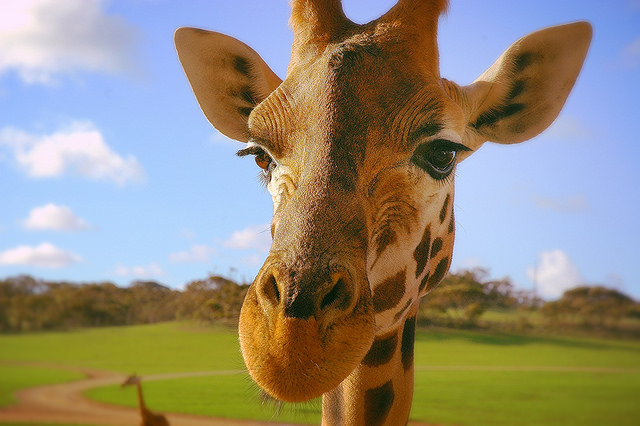
\includegraphics[width=.5\linewidth]{giraffe.jpg}
  \caption{An adorable Giraffe.}
\end{subfigure}%
\begin{subfigure}[b]{.5\textwidth}
  \centering
  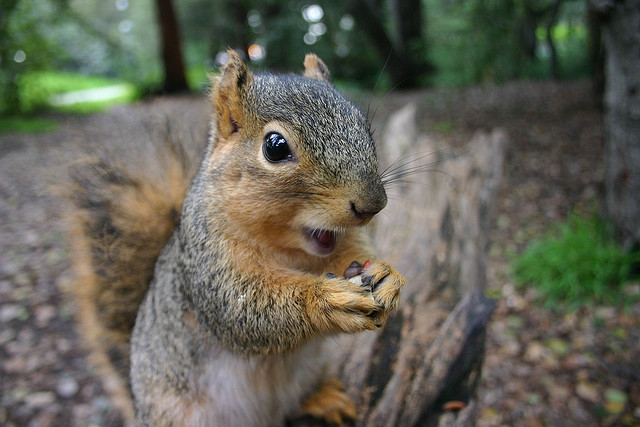
\includegraphics[width=.5\linewidth]{squirrel.jpg}
  \caption{An adorable Squirrel.}
\end{subfigure}
\caption{Adorable Animals.\label{fig:example}}
\end{figure}

In Figure~\ref{fig:example}, we have an example of images as sub-figures. Also animals.
\chapter{Conclusion}

Hopefully this example report is helpful.

\section{Section 1}

\subsection{Sub Section 1}

Some text here.

\subsection{Sub Section 2}

Moar text here.

\section{Section 2}

Fin.

\bibliographystyle{socreport}
\bibliography{report}

% Appendix (Remove if no appendix)
\appendix
\chapter{First appendix}
blah blah
\chapter{Second appendix}
blah blah

\end{document}
